\section{OPERATIONAL ROBUSTNESS STUDY}
\noindent A source-based methodological review identified corrective authority, confirmation, family-specific processing stages, review complexity and consequence valuation as unresolved assumptions. It was not independent human expert validation. We froze two one-factor changes, retaining the original condition at both base capacities, the same six policies and the frozen application estimator.\draftcredit

\subsection{Authority and Complexity Changes}
Under restricted authority, a completed review perfectly detects whether the staged proposal is wrong. A correct proposal is approved unchanged. A wrong proposal is blocked, leaving the account unchanged and the service unresolved. It is removed from the queue and cannot post later. Blocking counts neither as task completion nor correction. The preventable loss is therefore
\begin{equation}
 G_i^{\mathrm{block}}(T)=\ind[T\leq d_i]W_i.
 \label{eq:block}
\end{equation}
The missing service benefit is substantive. Since $W_i$ varies, replacing $4+W_i$ by $W_i$ is not a uniform rescaling and can change risk-weighted rankings. Perfect detection remains idealized, and labels are still unavailable before completed review.

The separate complexity condition retains full correction authority and uses
\begin{equation}
 s_i=s+\ind[\text{proposed item-list length}\geq 2],
 \label{eq:complexity}
\end{equation}
where $s$ is one or two ticks. This public proxy captures an additional item-checking burden without fitting review times. A mistaken omission may reduce the apparent complexity, which is retained as a limitation. Arrivals, cutoffs, consequence weights, preparation and risk remain unchanged. We do not evaluate an authority-by-complexity factorial design.

Two outcomes follow mathematically. No-review loss is invariant across variants. Under perfect blocking, every policy's correct-task count equals the initially correct staged count, since neither a wrong nor an unstaged request can be completed by blocking. These invariances are semantic checks rather than empirical discoveries.

\subsection{Fresh Source Cases and Analysis}
We audit all 500 train, 20 dev and 115 test records at the pinned revision, excluding all 120 Stage 5 accounts across source splits. Eligibility retains the original explicit-instruction, supported single-transaction criteria and source-intent consistency checks. Only ten unused eligible modification accounts remain, so a 16-bundle design is infeasible. The declared fallback selects eight globally disjoint bundles from 24 training cases, reserving modification first and then cancellation and returns/exchanges in source order. The source pool is not filtered using model outcomes or expected scheduling gains.

Three fresh replicates yield 72 workflow attempts. The same preparations feed six policies, two base durations and three operational variants, giving 864 policy episodes without repeated GPU calls for scheduling. The primary comparison is search minus greedy under restricted authority at base duration two. We average replicates within each of the eight bundles and use 2,000 common-index bootstrap draws with seed 20260916. Individual bundle differences accompany the interval. The same variants applied to the earlier 32 bundles are explicitly post hoc saved-data sensitivity, analyzed separately and never pooled with the fresh cases.

\subsection{Fresh Results}

All 72 workflow attempts are retained. Fifty-one stage a transaction, 39 are initially correct and 12 stage a wrong valid transaction. Twenty-one do not stage, comprising 18 step-limit failures and three finishes without a transaction. All 675 GPU generations succeed, with no retry. Table~\ref{tab:fresh} gives every policy and condition.

The primary restricted-authority difference is $+1.667$ loss points for search minus greedy, with a 95\% paired interval of $[0.000,4.667]$. Search wins on zero bundles, ties on six and loses on two. The eight bundle-mean differences in numerical order are $0,0,0,0,0,0,1.333,12.000$. The wide interval reflects a small, sparse sample and does not establish equivalence or a general population disadvantage.

Search blocks eight wrong transactions versus greedy's twelve and lets four wrong transactions post. Both complete 39 of 72 tasks because blocking cannot complete a wrong or unstaged request. Search performs 44 reviews versus 42, consuming 88 versus 84 ticks. Its loss is 172 points versus 132, or 7.167 versus 5.500 per three-case run. EDF has mean loss 7.000. The secondary search--EDF difference is $+0.167\;[0.000,0.500]$, with seven bundle ties and one loss.

\begin{table*}[t]

\caption{Fresh follow-up mean loss. Each cell represents 24 runs on eight source bundles. C and X are correct-task totals at base duration two for correction and complexity time, with denominator 72. Approve/block completes 39 tasks under every policy. No-review inputs are identical across conditions.}

\label{tab:fresh}\centering\small

\begin{tabular}{lrrrrrrrr}

\toprule

& \multicolumn{2}{c}{Correction} & \multicolumn{2}{c}{Approve/block} & \multicolumn{2}{c}{Complexity time} & \multicolumn{2}{c}{Correct} \\ Policy & 1 tick & 2 ticks & 1 tick & 2 ticks & 1 tick & 2 ticks & C & X \\

\midrule

No review & 9.833 & 9.833 & 9.833 & 9.833 & 9.833 & 9.833 & 39 & 39 \\

FCFS & 3.500 & 5.500 & 5.500 & 7.000 & 3.500 & 5.833 & 48 & 47 \\

EDF & 3.500 & 5.500 & 5.500 & 7.000 & 3.500 & 5.833 & 48 & 47 \\

Uncertainty & 3.500 & 3.500 & 5.500 & 5.500 & 3.500 & 3.833 & 51 & 50 \\

Greedy & 3.500 & 3.500 & 5.500 & 5.500 & 3.500 & 3.833 & 51 & 50 \\

Search & 3.500 & 5.833 & 5.500 & 7.167 & 3.500 & 6.167 & 47 & 46 \\

\bottomrule

\end{tabular}

\end{table*}



At one tick, every review policy prevents every staged error in all three variants. Correction and complexity time reach the 21-unstaged-failure floor of 84 loss points. Blocking instead retains unresolved service loss for all 33 initially unsuccessful requests, totaling 132 points. These distinct floors follow from corrective authority, not from a better scheduling rule.

At two ticks, full correction gives search minus greedy $+2.333\;[0.000,6.333]$. The complexity variant has the same paired difference while increasing both policies' loss by one third of a point. Only six staged proposals from four cases trigger the added tick, including two initially wrong proposals. This limited exposure bounds what the complexity null contrast establishes.

Approve/block leaves every fresh review sequence unchanged relative to correction. Its smaller search--greedy loss difference is therefore explained by the changed preventable consequence, not an observed improvement in allocation. The benefit functions can produce different rankings in arithmetic cases, but do not do so in these fresh trajectories.

\begin{figure*}[t]

\centering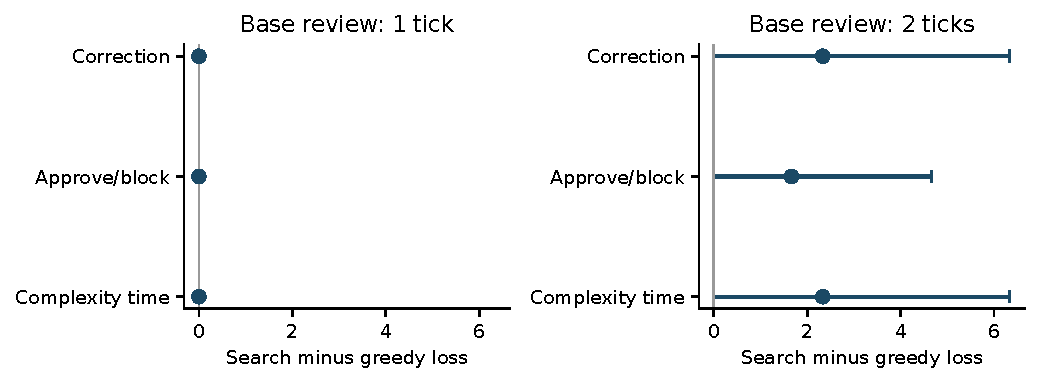
\includegraphics[width=0.98\textwidth]{../artifacts/stage6_robustness/analysis/fresh/figures/paired_loss.pdf}

\caption{Fresh operational sensitivity. Points are search minus greedy mean loss; bars are 95\% paired bundle-bootstrap intervals. Only approve/block at base duration two is primary. Degenerate one-tick intervals describe ties in this sample, not population equivalence.}

\label{fig:robustness}\end{figure*}

\subsection{Scheduling Mechanism and Error Ranking}

Search and greedy review sequences differ in six of 24 fresh runs at base duration two, versus one search--EDF difference. On search's states, 19 dispatches have multiple eligible requests and six have different greedy/search heads. These are repeated states for descriptive analysis, not additional independent observations.

The first unfavorable example is bundle 06, replicate 2. At tick zero, search reviews a correct cancellation with cutoff two, planning to preserve both currently available opportunities. Greedy instead blocks the wrong modification by tick two. A correct exchange arrives at tick one. When search becomes free, its frozen estimate prioritizes that exchange, and the modification posts at tick five. Search loss is eight versus greedy's four. The primary example rule finds no fresh search benefit. The first tie contains a blocked incomplete return and an unstaged modification, giving equal loss eight.

The frozen estimator's aggregate Brier score is 0.17144, versus 0.17998 for its pooled estimate; AUROC is 0.6581. Yet modification has eight errors among 13 staged proposals, versus four among 18 returns/exchanges, while predicted risks rank those families in the opposite order. All 20 staged cancellations are correct. This retrospective evidence helps explain the unfavorable trace without granting labels to the scheduler or refitting on evaluation data. Eight source cases produce different proposals across the three replicates, and four have mixed initial correctness.

\subsection{Saved-Preparation Sensitivity}

The separate post hoc analysis replays all 1,152 original reference traces exactly and adds the declared variants on the same 288 preparations. At base duration two, restricted-authority search minus greedy is $+0.125\;[-0.167,0.500]$, with one win, 29 ties and two losses. Complexity time gives $+0.500\;[-0.083,1.250]$, with one win, 28 ties and three losses. These results do not replace the original $+0.250$ primary comparison. Blocking changes search's actual sequence in only two of 96 runs relative to correction. The first saved-data benefit remains available as a trace alongside the fresh null and unfavorable examples.


